% !TeX TXS-program:compile = txs:///arara
% arara: lualatex: {shell: no, synctex: yes, interaction: batchmode}
% arara: pythontex: {rerun: modified} if found('pytxcode', 'PYTHONTEX#py')
% arara: lualatex: {shell: no, synctex: yes, interaction: batchmode} if found('pytxcode', 'PYTHONTEX#py')
% arara: lualatex: {shell: no, synctex: yes, interaction: batchmode} if found('log', '(undefined references|Please rerun|Rerun to get)')

\documentclass[a4paper,11pt]{article}
\usepackage[revgoku]{cp-base}
\graphicspath{{./graphics/}}
%variables
\donnees[%
	classe={1\up{ère} 2M2},
	matiere={[SPÉ.MATHS]},
	mois=Septembre,annee=2021,
	typedoc=EXOS~,
	numdoc=1,
	mois=Septembre,
	annee=2021
	]
%formatage
\author{Pierquet}
\title{\nomfichier}
\hypersetup{%
	pdfauthor={Pierquet},pdftitle={\nomfichier},allbordercolors=white,pdfborder=0 0 0,pdfstartview=FitH
	}
%divers
\lhead{\entete{\matiere}}
\chead{\entete{\lycee}}
\rhead{\entete{\classe{} - \mois{} \annee}}
\lfoot{\pied{\matiere}}
\cfoot{\logolycee{}}
\rfoot{\pied{\numeropagetot}}

\begin{document}

\pagestyle{fancy}

\part{CH01 - Polynômes du second degré - Exercices}

\medskip

\begin{caide}
	{\setlength\arrayrulewidth{1.5pt} \arrayrulecolor{titrebleu!35}
		\begin{tabularx}{\linewidth}{Y|Y|Y|Y|Y|Y}
			\niveaudif{0}~~\textsf{Basique} & \niveaudif{1}~~\textsf{Modérée} & \niveaudif{2}~~\textsf{Élevée} & \niveaudif{3}~~\textsf{Très élevée} & \niveaudif{4}~~\textsf{Extrême} & \niveaudif{5}~~\textsf{Insensée} \\
		\end{tabularx}\arrayrulecolor{black}}
\end{caide}

\medskip

\exonum{0}

\medskip

Les questions suivantes sont indépendantes.
\begin{enumerate}
	\item Dans chaque cas, écrire le trinôme sous sa forme canonique :
	\begin{enumerate}
		\item $x^2+6x-8$ ;
		\item $2x^2+6x+4$ ;
		\item $3x^2+12x+12$ ;
		\item $-x^2+7x-10$.
	\end{enumerate}
	\item Déterminer le tableau de variation des fonctions suivantes :
	\begin{enumerate}
		\item $f(x)=2(x-4)^2+3$ ;
		\item $g(x)=-3(x+1)^2-5$ ;
		\item $h(x)=x(x-8)$.
	\end{enumerate}
	\item Soit $f$ la fonction définie sur $\R$ par $f(x)=-2x^2+8x-13$.
	\begin{enumerate}
		\item Déterminer la forme canonique de la fonction $f$.
		\item En déduire le maximum de $f$ et la valeur de $x$ pour laquelle il est atteint.
	\end{enumerate}
\end{enumerate}

\medskip

\exonum{0}

\medskip

Les questions suivantes sont indépendantes.
\begin{enumerate}
	\item Résoudre, dans $\R$, les équations suivantes :
	\begin{enumerate}
		\item $x^2-x-6=0$ ;
		\item $x^2-x+2=0$ ;
		\item $-x^2+2x-1=0$ ;
		\item $x^2+x-1=0$ ;
		\item $2x^2+12x+18=0$ ;
		\item $x^2+x=-1$ ;
		\item $(2x-1)^2+3=0$.
	\end{enumerate}
	\item Écrire -- si possible -- les trinômes suivants sous la forme d'un produit de facteurs :
	\begin{enumerate}
		\item $f(x)=x^2-7x+10$ ;
		\item $g(x)=-3x^2+4x+4$ ;
		\item $h(x)=-\dfrac12 x^2 - \dfrac12x + 1$ ;
		\item $i(x)=2x^2+2x+2$.
	\end{enumerate}
\end{enumerate}

\newpage

\exonum{0}

\medskip

Sur le graphique suivant, on donne cinq paraboles.

Attribuer, en justifiant, à chacune de ces courbes la fonction qui lui est associée.

\begin{center}
	\tunits{1}{1}
	\tdefgrille{-5}{5}{1}{1}{-6}{7}{1}{1}
	\begin{tikzpicture}[x=\xunit cm,y=\yunit cm]
		%AXES & GRILLES
		\tgrilles[line width=0.4pt,color=lightgray] ;
		\axestikz ;
		\axextikz[size=\small]{-5,-4,...,4} ;
		\axeytikz[size=\small]{-6,-5,...,6} ;
		%LABELS
		\draw (5,2) node[right=4pt] {$f_1(x)=-x^2+2x-3$} ;
		\draw (5,1) node[right=4pt] {$f_2(x)=x^2+x+3$} ;
		\draw (5,0) node[right=4pt] {$f_3(x)=2x^2-5x+3$} ;
		\draw (5,-1) node[right=4pt] {$f_4(x)=-2x^2-5x+3$} ;
		\draw (5,-2) node[right=4pt] {$f_5(x)=x^2+x+\tfrac14$} ;
		%COURBES
		\clip (\xmin,\ymin) rectangle (\xmax,\ymax) ;
		\draw[line width=1.5pt,blue,domain=-5:5,samples=200] plot(\x,{-\x*\x+2*\x-3});
		\draw[line width=1.5pt,red,domain=-5:5,samples=200] plot(\x,{\x*\x+\x+3});
		\draw[line width=1.5pt,purple,domain=-5:5,samples=200] plot(\x,{2*\x*\x-5*\x+3});
		\draw[line width=1.5pt,ForestGreen,domain=-5:5,samples=200] plot(\x,{-2*\x*\x-5*\x+3});
		\draw[line width=1.5pt,orange,domain=-5:5,samples=200] plot(\x,{\x*\x+\x+0.25});
	\end{tikzpicture}
\end{center}

\medskip

\exonum{2}

\medskip

Les questions suivantes sont \textit{indépendantes}.
\begin{enumerate}
	\item Résoudre, dans $\R$, les équations (on transformera si besoin !) :
	\begin{enumerate}
		\item $x^3-8x^2+18x=0$ ;
		\item $\dfrac{x^2+2x+1}{x+1}=2x-1$ ;
		%\item $\dfrac{1}{x+2}-\dfrac{2}{2x-5}=\dfrac94$ ;
		\item $\dfrac{3x^2+10x+8}{x+2}=2x+5$.
	\end{enumerate}
	\item On considère l'équation $x^2-4x+(m-1)=0$ où $m$ est un paramètre.
	\begin{enumerate}
		\item Pour quelle valeur de $m$ l'équation admet-elle une seule racine (double) ?
		\item Calculer cette racine.
	\end{enumerate}
%	\item Soit $m \in \R$ et soit $f$ la fonction du second degré définie par $f(x)=x^2-(m+1)x+4$.
%	\begin{enumerate}
%		\item Pour quelle(s) valeur(s) de $m$ l'équation $f(x)=0$ a-t-elle une seule solution ?
%		
%		Calculer alors cette solution.
%		\item Pour quelle(s) valeur(s) de $m$ l'équation $f(x)=0$ n'a-t-elle aucune solution ?
%	\end{enumerate}
	\item On considère l'équation $x^2-5x+6=0$.
	\begin{enumerate}
		\item Vérifier que 2 est solution de cette équation.
		\item Quelle est la somme et le produit des racines ?
		\item En déduire l'autre solution.
	\end{enumerate}
	\item Résoudre les systèmes suivants :
	\begin{enumerate}
		\item $\begin{dcases} x+y=18 \\xy=65 \end{dcases}$ ;
		\item $\begin{dcases} x+y=4 \\xy=5 \end{dcases}$.
	\end{enumerate}
\end{enumerate}

\medskip

\exonum{2}

\medskip

Peut-on trouver trois carrés ayant pour côtés des entiers \textit{consécutifs} et dont la somme des aires est 15\,125 ?

Si oui préciser quelles sont les valeurs que doivent avoir les côtés.

Même question avec 15\,127.

\begin{center}
	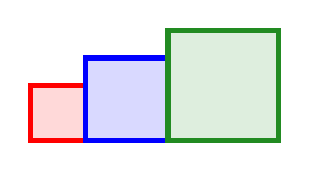
\begin{tikzpicture}[scale=0.35]
		\draw[line width=2pt,red,fill=red!15] (0,0) rectangle (2,2) ;
		\draw[line width=2pt,blue,fill=blue!15] (2,0) rectangle (5,3) ;
		\draw[line width=2pt,ForestGreen,fill=ForestGreen!15] (5,0) rectangle (9,4) ;
	\end{tikzpicture}
\end{center}
%
%\begin{center}
%	\psset{unit=1cm,linewidth=2pt}
%	\begin{pspicture}(9,4)
%		\psframe[linecolor=red,fillstyle=solid,fillcolor=red!15](0,0)(2,2)
%		\psframe[linecolor=blue,fillstyle=solid,fillcolor=blue!15](2,0)(5,3)
%		\psframe[linecolor=ForestGreen,fillstyle=solid,fillcolor=ForestGreen!15](5,0)(9,4)
%	\end{pspicture}
%\end{center}

\medskip

\exonum{2}

\medskip

Quelle largeur doit-on donner à la croix pour que son aire soit égale à l’aire restante du drapeau ?

\begin{center}
	\tikzset{gras/.style={line width=1.5pt}}
	\tikzset{fin/.style={line width=0.75pt}}
	\begin{tikzpicture}[x=1.5 cm,y=1.5cm,scale=0.75]
		\draw[gras] (0,0) rectangle (5,3) ;
		\draw[gras,fill=gray!25] (0,0) rectangle (1.5,0.8) ;
		\draw[gras,fill=gray!25] (2.1,0) rectangle (5,0.8) ;
		\draw[gras,fill=gray!25] (0,1.4) rectangle (1.5,3) ;
		\draw[gras,fill=gray!25] (2.1,1.4) rectangle (5,3) ;
		\draw[gras,<->] (0,-0.3) -- (5,-0.3) ;
		\draw (2.5,-0.3) node[below] {\textsf{4~m}} ;
		\draw[fin] (0,0) -- (0,-0.3) (5,0) -- (5,-0.3) ;
		\draw[<->,gras] (5.3,0) -- (5.3,3) ;
		\draw (5.3,1.5) node[right] {\textsf{3~m}};
		\draw[fin](5,0)--(5.3,0) (5,3)--(5.3,3);
		\draw[<->,gras](-0.3,0.8)--(-0.3,1.4);
		\draw (-0.3,1.1) node[left] {$\mathsf{x}$};
		\draw[fin](-0.3,1.4)--(0,1.4) (-0.3,0.8)--(0,0.8);
		\draw[<->,gras](1.5,3.3)--(2.1,3.3);
		\draw (1.8,3.3) node[above] {$\mathsf{x}$};
		\draw[fin](1.5,3)--(1.5,3.3) (2.1,3)--(2.1,3.3);
	\end{tikzpicture}
\end{center}
%
%\exonum{2}
%
%\medskip
%
%On dispose d’une baguette de bois de 10~cm de long.
%\begin{enumerate}
%	\item Où briser la baguette pour que les morceaux obtenus soient les \textit{deux côtés consécutifs} d’un rectangle de surface 20~cm\up{2} ?
%	\begin{center}
%		\tunits{1.25}{1.25}
%		\tikzset{baton/.style={line width=3pt,brown}}
%		\begin{tikzpicture}[x=\xunit cm,y=\yunit cm,scale=0.75]
%			\draw[line width=1.5pt,fill=gray!25] (7,0) rectangle (11,2);
%			\draw (9,1) node {\large \textsf{20~cm\up{2}}};
%			\draw[baton] (0,2)--(6,2) (7,0)--(7,2)--(11,2);
%			\draw[line width=1.5pt,<->] (0,1.6) -- (6,1.6);
%			\draw (3,1.6) node[below] {\large \textsf{10~cm}};
%		\end{tikzpicture}
%	\end{center}
%%	\begin{center}
%%		\psset{unit=1.25cm,linewidth=1.5pt}
%%		\begin{pspicture}[](0,0)(11,2)
%%			\psframe[fillstyle=solid,fillcolor=gray!25](7,0)(11,2)
%%			\rput(9,1){\large \textsf{20~cm\up{2}}}
%%			\psline[linewidth=3pt,linecolor=brown](0,2)(6,2)
%%			\psline{<->}(0,1.6)(6,1.6)\uput[d](3,1.6){\large \textsf{10~cm}}
%%			\psline[linewidth=3pt,linecolor=brown](7,0)(7,2)(11,2)
%%		\end{pspicture}
%%	\end{center}
%	\item Même question pour avoir un rectangle de 40 cm\up{2} ?
%\end{enumerate}

\medskip

\exonum{2}

\medskip

Créer une \calg{procédure}, en \calgpython, qui :

\begin{itemize}
	\item prendra en \calg{paramètres} les coefficients \calg{a}, \calg{b} et \calg{c} d'un trinôme $ax^2+bx+c$ ;
	\item affichera les coordonnées du sommet de la parabole représentant le trinôme ;
	\item indiquera également l'orientation de cette parabole
\end{itemize}

\begin{pyconcode}
# Calcul de alpha et de beta
from math import *
def analysetrinome(a,b,c):
	alpha = -b/(2*a)
	beta = a*alpha**2 + b*alpha + c
	print(f"Le sommet de la parabole a pour coordonnées ({alpha},{beta})")
	if a > 0 :
		print("La parabole est ouverte vers le haut")
	else :
		print("La parabole est ouverte vers le bas")

\end{pyconcode}

\begin{tcpythoncodeno}[15cm]
	\begin{pyverbatim}[][fontsize=\footnotesize,numbers=none]
		def analysetrinome(a,b,c) :
			alpha = .....
			beta = ......
			print(f"Le sommet de la parabole a pour coordonnées ..........")
			if a ...... :
				print(......)
			else :
				print(......)
	\end{pyverbatim}
\end{tcpythoncodeno}

On devra avoir, par exemple :

\begin{consolepython}[15cm]
\begin{pyconsole}[][framesep=3mm,frame=single,label={[\scriptsize Début de la console \logopython]\scriptsize Fin de la console \logopython},fontsize=\footnotesize,framerule=1pt,rulecolor=\color{ForestGreen}]
analysetrinome(-1,2,-3)
\end{pyconsole}
\end{consolepython}
\end{document}